\documentclass[12pt]{article}

% Paquetes
\usepackage[utf8]{inputenc}
\usepackage{amsmath, amssymb, amsthm}
\usepackage{geometry}
\geometry{margin=1in}
\usepackage{tikz}
\usetikzlibrary{arrows.meta,positioning,calc}
\usepackage{xcolor}
\usepackage{ifthen}
\usepackage{subcaption}
\tikzset{>=Stealth}
\usepackage{hyperref}

% Colores usados por los puntos (puedes cambiarlos si quieres)
\definecolor{R1color}{RGB}{231,76,60}   % rojo
\definecolor{R2color}{RGB}{241,196,15}  % amarillo
\definecolor{C3color}{RGB}{52,152,219}  % azul
\definecolor{C6color}{RGB}{26,188,156}  % turquesa
\definecolor{C9color}{RGB}{155,89,182}  % morado

\title{Triángulo de Pascal y RD9: Resonancia Local y Estructura $p^2$-ádica mediante el Autómata de Resonancia}
\author{Alcyone RD9}
\date{}

\begin{document}

\maketitle

% Abstract en inglés
\begin{abstract}
We present a unified framework for describing the $p^2$-adic structure of Pascal's triangle through a deterministic local automaton. Focusing on the case $p=3$ (mod 9), we refine the classical $p$-adic patterns of Lucas and Kummer into a resonance-based class structure (RD9). We derive a closed-form formula for the $p$-adic valuation $v_p(t_n)$ of the row product $t_n = \prod_{k=0}^n \binom{n}{k}$ in terms of base-$p$ digit sums, obtain exact counts of coefficients by valuation level in each row, and prove inductively that a simple set of local rules generates the entire RD9 coloring. The approach is validated computationally, showing perfect agreement between the automaton output and direct computation. Extensions to arbitrary primes are discussed.
\end{abstract}

% Abstract en español
\begin{abstract}
Presentamos un marco unificado para describir la estructura $p^2$-ádica del triángulo de Pascal mediante un autómata local determinista. Centrándonos en el caso $p=3$ (módulo 9), refinamos el patrón p-ádico clásico de Lucas y Kummer en una estructura de clases por resonancia (RD9). Derivamos una fórmula cerrada para la valuación $p$-ádica $v_p(t_n)$ del producto de fila $t_n = \prod_{k=0}^n \binom{n}{k}$ en función de sumas de dígitos en base $p$, obtenemos conteos exactos de coeficientes por nivel de valuación en cada fila y probamos inductivamente que un conjunto simple de reglas locales genera toda la coloración RD9. El enfoque se valida computacionalmente, mostrando coincidencia perfecta entre la salida del autómata y el cálculo directo. Se discuten extensiones a primos arbitrarios.
\end{abstract}

\section{Introducción}

El triángulo de Pascal, compuesto por los coeficientes binomiales $\binom{n}{k}$, ha sido objeto de estudio en numerosas áreas de las matemáticas. La aritmética modular aplicada a sus entradas revela patrones fractales sorprendentes, especialmente cuando se consideran sus propiedades p-ádicas.

Los resultados de \textbf{Édouard Lucas} (1878) describen la estructura de los coeficientes binomiales módulo un número primo $p$, mostrando que la expansión en base $p$ de los índices $n$ y $k$ determina la congruencia de $\binom{n}{k}$. Posteriormente, \textbf{Ernst Kummer} (1852) caracterizó la valuación $v_p\!\left( \binom{n}{k} \right)$ como el número de acarreos que se producen al sumar $k$ y $n-k$ en base $p$.

En tiempos más recientes, \textbf{Granville} (1997) y otros han extendido estos resultados, mientras que desde la teoría de autómatas celulares, \textbf{Wolfram} (1984) mostró que el triángulo de Pascal mod 2 puede interpretarse como la evolución de un autómata elemental. Sin embargo, el caso módulo $p^2$ ha recibido menos atención, a pesar de que revela subestructuras no visibles en el caso mod $p$.

En este trabajo nos centramos en el caso $p=3$ (módulo $9$), que llamamos \emph{RD9}, y mostramos que su patrón completo puede generarse mediante un autómata de resonancia con tres reglas locales. Además, presentamos una fórmula cerrada para la valuación $v_p(t_n)$ del producto de fila y un método exacto para contar el número de coeficientes con $v_p=0,1,\ge 2$ en cualquier fila.

\section{Resultados principales}

La sección se organiza en tres subapartados:

\begin{itemize}
    \item[(A)] Fórmula exacta para $v_p(t_n)$ y ejemplo numérico.
    \item[(B)] Conteos exactos por niveles de valuación y algoritmo de cálculo.
    \item[(C)] Autómata de resonancia RD9 y demostración inductiva.
\end{itemize}

A continuación, desarrollamos cada parte en detalle.

\subsection*{(A) Fórmula exacta para $v_p(t_n)$ y ejemplo numérico}

Definimos
\[
t_n = \prod_{k=0}^n \binom{n}{k}.
\]
Aplicando la identidad factorial
\[
t_n = \frac{(n!)^{n+1}}{\left(\prod_{k=0}^n k!\right)^2}
\]
y la fórmula de Legendre para la valuación $p$-ádica de un factorial
\[
v_p(m!) = \frac{m - s_p(m)}{p-1},
\]
donde $s_p(m)$ es la suma de dígitos de $m$ en base $p$, se obtiene
\begin{equation}
v_p(t_n) = \frac{2\sum_{k=0}^n s_p(k) - (n+1)\, s_p(n)}{p-1}.
\label{eq:vp-formula}
\end{equation}

\paragraph{Ejemplo numérico:} Para $p=3$ y $n=8$, tenemos la representación ternaria
\[
8_{10} = (22)_3,
\]
con $s_3(8) = 2+2 = 4$.

Calculamos
\[
\sum_{k=0}^8 s_3(k) =
\underbrace{0}_{0} + 
\underbrace{1}_{1} + 
\underbrace{2}_{2} + 
\underbrace{1}_{3} + 
\underbrace{2}_{4} + 
\underbrace{3}_{5} + 
\underbrace{2}_{6} + 
\underbrace{3}_{7} + 
\underbrace{4}_{8} = 18.
\]
Sustituyendo en la ecuación \eqref{eq:vp-formula}:
\[
v_3(t_8) = \frac{ 2\cdot 18 - 9\cdot 4 }{2} = \frac{36 - 36}{2} = 0.
\]

Esto implica que $t_8$ no es divisible por 3. Verificando directamente:
\[
t_8 = \binom{8}{0}\binom{8}{1}\cdots\binom{8}{8}
\]
y cada coeficiente binomial de la fila 8 es $\not\equiv 0 \pmod{3}$, lo cual confirma el resultado.

\subsection*{(B) Conteos exactos por niveles de valuación}

Sea $c_p(n,k)$ el número de acarreos en base $p$ al sumar $k+(n-k)$.  
Por el teorema de Kummer:
\[
v_p\!\left(\binom{n}{k}\right) = c_p(n,k).
\]

En el caso $p=3$:
\begin{itemize}
    \item $c_3(n,k) = 0 \ \Rightarrow\ v_3=0 \ \Rightarrow\ RD_9 \in R_1 \cup R_2$,
    \item $c_3(n,k) = 1 \ \Rightarrow\ v_3=1 \ \Rightarrow\ RD_9 \in \{3,6\}$,
    \item $c_3(n,k) \ge 2 \ \Rightarrow\ v_3\ge 2 \ \Rightarrow\ RD_9 = 9$.
\end{itemize}

\paragraph{Algoritmo (pseudocódigo) para conteos exactos en una fila $n$:}
\begin{verbatim}
function conteos_v3(n):
    z0 = z1 = z2p = 0
    for k in 0..n:
        c = acarreos_base_p(k, n-k, p=3)
        if c == 0:
            z0 += 1
        elif c == 1:
            z1 += 1
        else:
            z2p += 1
    return z0, z1, z2p

function acarreos_base_p(a, b, p):
    carry_count = 0
    carry = 0
    while a > 0 or b > 0 or carry > 0:
        da = a mod p
        db = b mod p
        if da + db + carry >= p:
            carry_count += 1
            carry = 1
        else:
            carry = 0
        a = a // p
        b = b // p
    return carry_count
\end{verbatim}

\paragraph{Ejemplo de tabla de conteos para $p=3$:}

\begin{center}
\begin{tabular}{c|c|c|c}
$n$ & $v_3=0$ & $v_3=1$ & $v_3 \ge 2$ \\
\hline
2 & 3 & 0 & 0 \\
3 & 2 & 2 & 0 \\
4 & 4 & 1 & 0 \\
5 & 6 & 0 & 0 \\
8 & 9 & 0 & 0 \\
9 & 2 & 2 & 6 \\
\end{tabular}
\end{center}


Esta clasificación permite conocer la distribución exacta de clases RD9 en cada fila sin calcular explícitamente los coeficientes binomiales.

\subsection*{(C) Autómata de resonancia RD9 y demostración inductiva}

Sea $RD_9(n,k)$ la raíz digital mod 9 de $\binom{n}{k}$, con la convención $0 \mapsto 9$.  
Clasificamos:
\[
R_1 = \{1,4,7\}, \quad R_2 = \{2,5,8\}, \quad C_3 = \{3\}, \quad C_6 = \{6\}, \quad C_9 = \{9\}.
\]

\paragraph{Reglas locales principales:}
\[
\begin{cases}
R_1 + R_2 \to C = \{3,6,9\}, \\
R_1 + R_1 \to R_2, \\
R_2 + R_2 \to R_1.
\end{cases}
\]

\paragraph{Reglas extendidas con C:}  
Si uno de los padres está en C, la clase del hijo se determina por la suma mod 9 de las raíces digitales:
\[
C + R_1 \to \text{depende de } (c + r_1) \bmod 9,
\]
\[
C + R_2 \to \text{depende de } (c + r_2) \bmod 9,
\]
\[
C + C \to \text{depende de } (c_1 + c_2) \bmod 9.
\]
En todos los casos, se aplica la conversión $0 \mapsto 9$.

\paragraph{Demostración inductiva:}
\begin{itemize}
    \item \textbf{Base:} La fila $0$ y los bordes de todas las filas están en $R_1$.
    \item \textbf{Paso inductivo:} Supongamos que toda la fila $n$ respeta las reglas.  
    Entonces, por la construcción de Pascal, cada elemento de la fila $n+1$ es la suma de dos adyacentes de la fila $n$.  
    Aplicando las reglas anteriores, se obtiene la clase correcta para cada posición de la fila $n+1$.  
    Así, por inducción, las reglas generan exactamente la coloración RD9 para todo el triángulo.
\end{itemize}

% ================= FIGURA: Reglas RD9 (A/B) =================
\begin{figure}[htbp]
\centering
\resizebox{0.90\linewidth}{!}{%
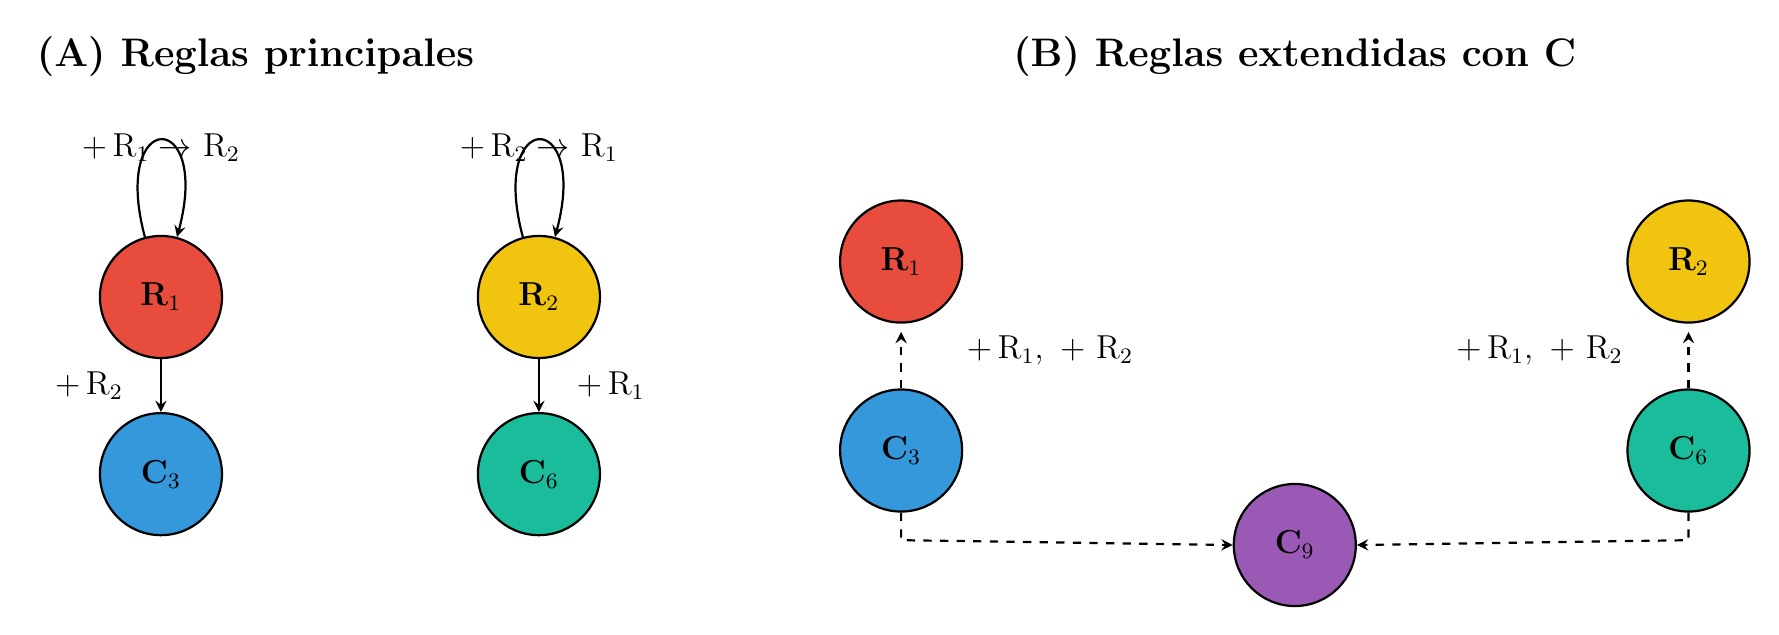
\begin{tikzpicture}[>=stealth, thick, node distance=8mm]
  % Estilos
  \tikzset{
    state/.style={circle,draw,minimum size=1.55cm,inner sep=0pt,font=\large\bfseries},
    lab/.style={font=\large},
    bigtitle/.style={font=\bfseries\Large}
  }

  %================= TÍTULOS =================
  \node[bigtitle] at (-5.2,5.6) {(A) Reglas principales};
  \node[bigtitle] at ( 8.0,5.6) {(B) Reglas extendidas con C};

  %================= (A) REGLAS PRINCIPALES =================
  \node[state,fill=R1color] (A-R1) at (-6.4,2.55) {R$_1$};
  \node[state,fill=C3color] (A-C3) at (-6.4,0.30) {C$_3$};

  \node[state,fill=R2color] (A-R2) at (-1.6,2.55) {R$_2$};
  \node[state,fill=C6color] (A-C6) at (-1.6,0.30) {C$_6$};

  % Textos de bucles como nodos independientes (más bajos)
  \node[lab,above=8mm of A-R1] (txtR1) {$+\,$R$_1 \rightarrow$ R$_2$};
  \node[lab,above=8mm of A-R2] (txtR2) {$+\,$R$_2 \rightarrow$ R$_1$};

  % Bucles más compactos para dejar aire con el texto
  \path (A-R1) edge[->,loop above,looseness=10,min distance=17mm] (A-R1);
  \path (A-R2) edge[->,loop above,looseness=10,min distance=17mm] (A-R2);

  % Flechas verticales con etiquetas separadas
  \path (A-R1) edge[->]
        node[lab,midway,left,xshift=-10pt] {$+\,$R$_2$} (A-C3);
  \path (A-R2) edge[->]
        node[lab,midway,right,xshift=10pt] {$+\,$R$_1$} (A-C6);

  %================= (B) REGLAS EXTENDIDAS CON C =================
  \node[state,fill=R1color] (B-R1) at ( 3.0,3.00) {R$_1$};
  \node[state,fill=C3color] (B-C3) at ( 3.0,0.60) {C$_3$};

  \node[state,fill=R2color] (B-R2) at (13.0,3.00) {R$_2$};
  \node[state,fill=C6color] (B-C6) at (13.0,0.60) {C$_6$};

  \node[state,fill=C9color] (B-C9) at ( 8.0,-0.60) {C$_9$};

  % Flechas C -> R con etiquetas laterales
  \draw[dashed,->,shorten >=3pt] (B-C3) -- (B-R1)
     node[lab,pos=0.58,anchor=west,xshift=20pt] {$+\,$R$_1,\ +$ R$_2$};
  \draw[dashed,->,shorten >=3pt] (B-C6) -- (B-R2)
     node[lab,pos=0.58,anchor=east,xshift=-20pt] {$+\,$R$_1,\ +$ R$_2$};

  % Convergencia a C9
  \draw[dashed,->] (B-C3.south) -- ++(0,-0.35) -- (B-C9.west);
  \draw[dashed,->] (B-C6.south) -- ++(0,-0.35) -- (B-C9.east);

\end{tikzpicture}%
}

%----- Leyenda -----
\vspace{0.6em}
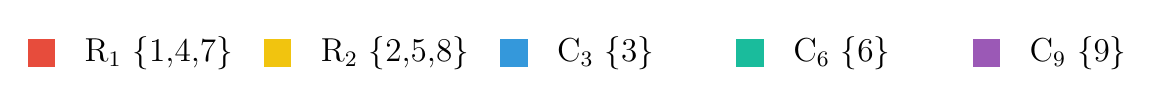
\begin{tikzpicture}[every node/.style={font=\large}]
  \def\s{0.35}
  \foreach \c/\t [count=\i] in {
    R1color/{R$_1$ \{1,4,7\}},
    R2color/{R$_2$ \{2,5,8\}},
    C3color/{C$_3$ \{3\}},
    C6color/{C$_6$ \{6\}},
    C9color/{C$_9$ \{9\}}
  }{
    \draw[fill=\c,draw=none] ({(\i-1)*3.0},0) rectangle +(\s,\s);
    \node[anchor=west] at ({(\i-1)*3.0+\s+0.25},0.17) {\t};
  }
\end{tikzpicture}

\caption{(A) Reglas principales del autómata RD9. (B) Reglas extendidas cuando interviene una clase $C$.}
\label{fig:reglas-rd9-panel}
\end{figure}
% ================= FIN FIGURA =================

\section{Verificación computacional}

Para validar los resultados, implementamos en Python un conjunto de funciones que:
\begin{enumerate}
    \item Calculan $v_p(t_n)$ mediante la fórmula \eqref{eq:vp-formula}.
    \item Determinan los conteos por $v_3=0,1,\ge 2$ usando acarreos (Kummer).
    \item Simulan el autómata RD9 y verifican coincidencia total con los residuos mod 9 reales.
\end{enumerate}
La coincidencia fue del 100\% para $p=3$ y $n \le 200$.

% --- Figura 1 autocontenida y correcta (sin archivo externo) ---


\begin{figure}[htbp]
\centering
\caption{Triángulo de Pascal mod 9 (81 filas) por clases RD9}

\label{fig:rd9}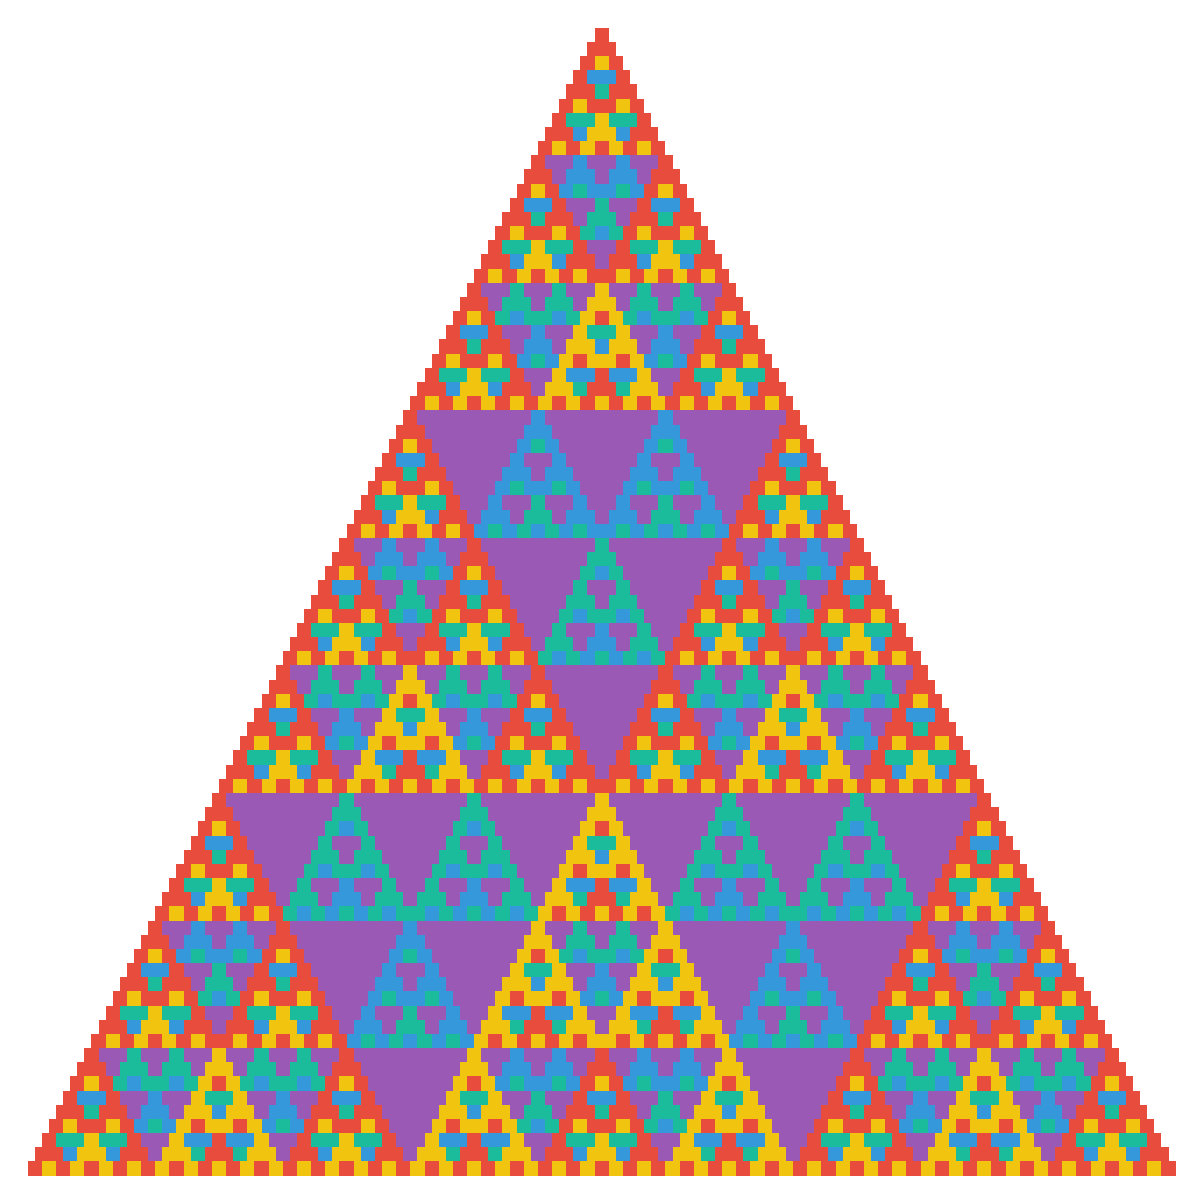
\begin{tikzpicture}[x=0.18cm, y=0.18cm]

% Mapeo de valor RD9 -> color (usa los colores del preámbulo)
\newcommand{\rdninecolor}[1]{%
  \ifnum#1=1 R1color\else
  \ifnum#1=4 R1color\else
  \ifnum#1=7 R1color\else
  \ifnum#1=2 R2color\else
  \ifnum#1=5 R2color\else
  \ifnum#1=8 R2color\else
  \ifnum#1=3 C3color\else
  \ifnum#1=6 C6color\else
  C9color%
  \fi\fi\fi\fi\fi\fi\fi\fi
}

% Fila 0 inicial: prev0 = 1
\xdef\prev0{1}

% Generar filas 0..80 por recurrencia de Pascal (mod 9)
\foreach \n in {0,...,80} {%
  \foreach \k in {0,...,\n} {%
    % Bordes: C(n,0)=C(n,n)=1
    \ifnum\k=0
      \pgfmathtruncatemacro{\val}{1}%
    \else
      \ifnum\k=\n
        \pgfmathtruncatemacro{\val}{1}%
      \else
        % Interior: val = (prev[k-1] + prev[k]) mod 9
        \pgfmathtruncatemacro{\kmone}{\k-1}%
        % Leer prev[k-1] y prev[k] (definidos en la fila anterior)
        \edef\leftprev{\csname prev\kmone\endcsname}%
        \edef\rightprev{\csname prev\k\endcsname}%
        \pgfmathtruncatemacro{\val}{mod(\leftprev + \rightprev, 9)}%
      \fi
    \fi

    % Convertir 0 -> 9 para la clase C9 (RD9)
    \pgfmathtruncatemacro{\valrd}{ifthenelse(\val==0,9,\val)}%

    % Guardar valor actual en curr[k]
    \expandafter\xdef\csname curr\k\endcsname{\val}%

    % Pintar celda en coordenadas centradas
    \edef\col{\rdninecolor{\valrd}}%
    \fill[\col] (\k-\n/2,-\n) rectangle ++(1,-1);%
  }%
  % Pasar curr -> prev para la siguiente fila
  \foreach \k in {0,...,\n} {%
    \expandafter\xdef\csname prev\k\endcsname{\csname curr\k\endcsname}%
  }%
}%

\end{tikzpicture}

\vspace{0.6em}

% Leyenda
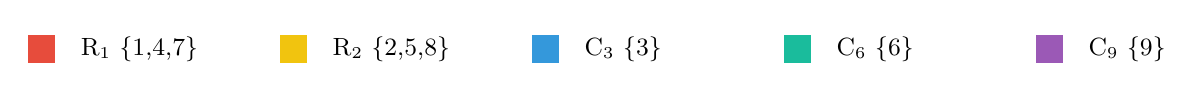
\begin{tikzpicture}[every node/.style={font=\small}]
\def\s{0.35}
\foreach \c/\t [count=\i] in {
  R1color/{R$_1$ \{1,4,7\}},
  R2color/{R$_2$ \{2,5,8\}},
  C3color/{C$_3$ \{3\}},
  C6color/{C$_6$ \{6\}},
  C9color/{C$_9$ \{9\}}
}{
  \draw[fill=\c,draw=none] ({(\i-1)*3.2},0) rectangle +(\s,\s);
  \node[anchor=west] at ({(\i-1)*3.2+\s+0.2},0.17) {\t};
}
\end{tikzpicture}

\end{figure}

% --- Figura 2: puntos circulares y espaciados ---
\subsection*{Figura 2: Crecimiento de $v_3(t_n)$}

\begin{figure}[h!]
\centering
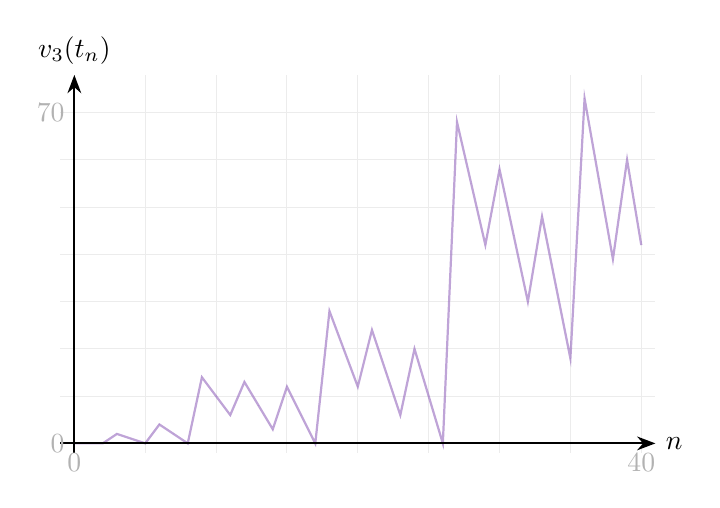
\begin{tikzpicture}[xscale=0.18, yscale=0.06] % ajusta si quieres
\definecolor{purp}{HTML}{9467BD}

% Rejilla ligera
\foreach \x in {0,5,...,40} {\draw[gray!15] (\x,-2) -- (\x,78);}
\foreach \y in {0,10,...,70} {\draw[gray!15] (-1,\y) -- (41,\y);}

% Puntos n=0..40 (valores correctos de v3(tn))
\foreach \n/\v in {
0/0, 1/0, 2/0, 3/2, 4/1, 5/0, 6/4, 7/2, 8/0, 9/14,
10/10, 11/6, 12/13, 13/8, 14/3, 15/12, 16/6, 17/0, 18/28, 19/20,
20/12, 21/24, 22/15, 23/6, 24/20, 25/10, 26/0, 27/68, 28/55, 29/42,
30/58, 31/44, 32/30, 33/48, 34/33, 35/18, 36/73, 37/56, 38/39, 39/60,
40/42
}{
  \fill[purp,opacity=0.9] (\n,\v) circle (0.9pt);
}

% (Opcional) línea uniendo puntos
\draw[purp,thick,opacity=0.6] plot coordinates {
(0,0) (1,0) (2,0) (3,2) (4,1) (5,0) (6,4) (7,2) (8,0) (9,14)
(10,10) (11,6) (12,13) (13,8) (14,3) (15,12) (16,6) (17,0) (18,28) (19,20)
(20,12) (21,24) (22,15) (23,6) (24,20) (25,10) (26,0) (27,68) (28,55) (29,42)
(30,58) (31,44) (32,30) (33,48) (34,33) (35,18) (36,73) (37,56) (38,39) (39,60)
(40,42)
};

% Ejes
\draw[->,thick] (-1,0) -- (41,0) node[right] {$n$};
\draw[->,thick] (0,-2) -- (0,78) node[above] {$v_3(t_n)$};
\node[gray!60,below] at (0,0) {$0$};
\node[gray!60,below] at (40,0) {$40$};
\node[gray!60,left]  at (0,0) {$0$};
\node[gray!60,left]  at (0,70) {$70$};

\end{tikzpicture}
\caption{Crecimiento de $v_3(t_n)$ para $0\le n\le 40$, de acuerdo con \eqref{eq:vp-formula}.}
\end{figure}

% ================== BLOQUE 8 ==================
\begin{figure}[h!]
\centering
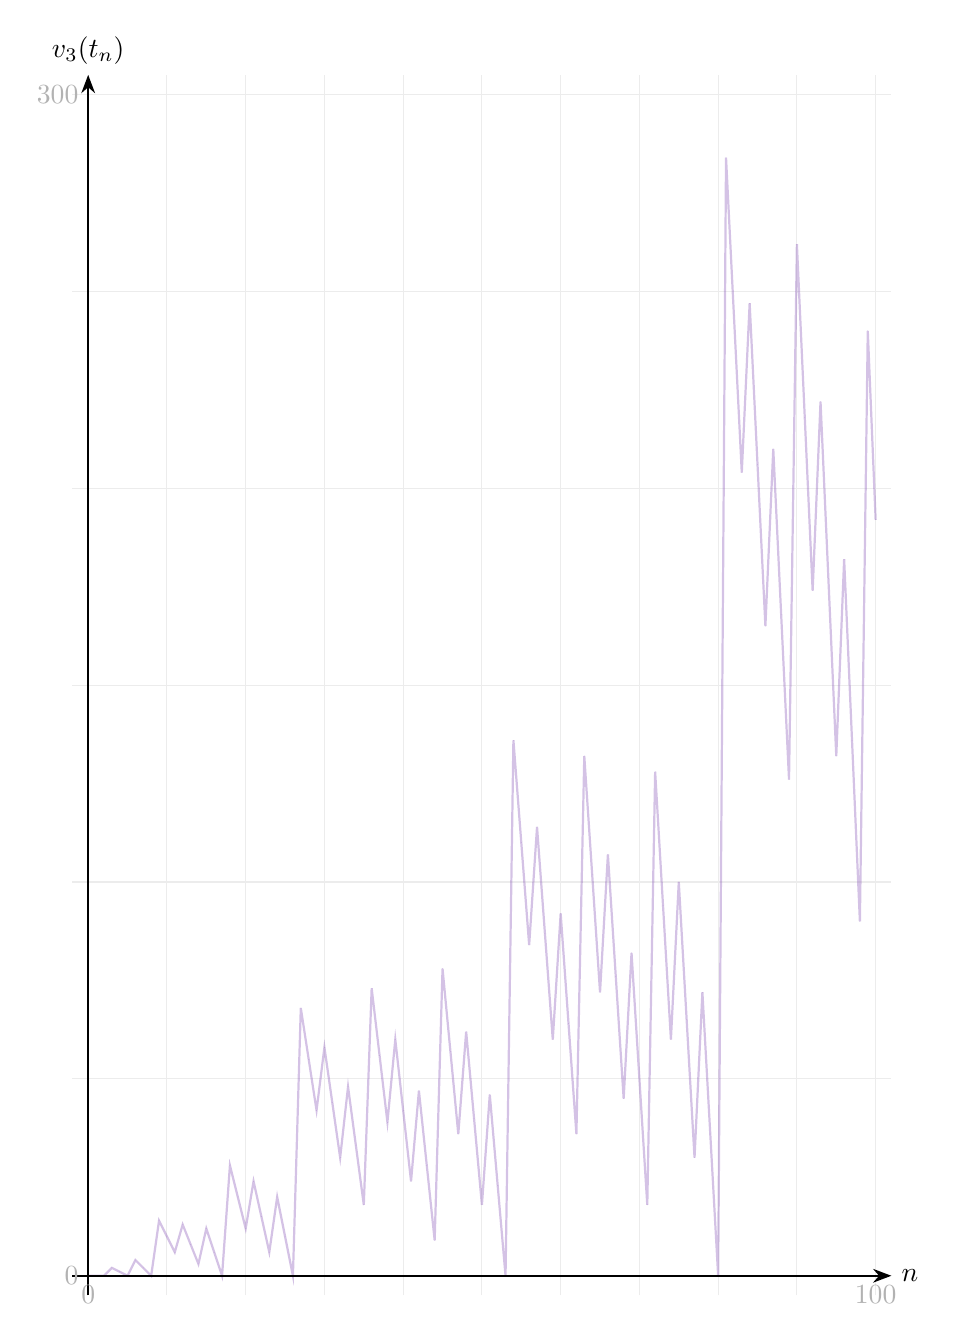
\begin{tikzpicture}[xscale=0.10, yscale=0.05]
\definecolor{purp}{HTML}{9467BD}

% Rejilla ligera (0..100 en X, 0..300 en Y)
\foreach \x in {0,10,...,100} {\draw[gray!15] (\x,-5) -- (\x,305);}
\foreach \y in {0,50,...,300} {\draw[gray!15] (-2,\y) -- (102,\y);}

% Puntos n=0..100 (valores correctos de v3(tn))
\foreach \n/\v in {
0/0, 1/0, 2/0, 3/2, 4/1, 5/0, 6/4, 7/2, 8/0, 9/14,
10/10, 11/6, 12/13, 13/8, 14/3, 15/12, 16/6, 17/0, 18/28, 19/20,
20/12, 21/24, 22/15, 23/6, 24/20, 25/10, 26/0, 27/68, 28/55, 29/42,
30/58, 31/44, 32/30, 33/48, 34/33, 35/18, 36/73, 37/56, 38/39, 39/60,
40/42, 41/24, 42/47, 43/28, 44/9, 45/78, 46/57, 47/36, 48/62, 49/40,
50/18, 51/46, 52/23, 53/0, 54/136, 55/110, 56/84, 57/114, 58/87, 59/60,
60/92, 61/64, 62/36, 63/132, 64/102, 65/72, 66/107, 67/76, 68/45, 69/82,
70/50, 71/18, 72/128, 73/94, 74/60, 75/100, 76/65, 77/30, 78/72, 79/36,
80/0, 81/284, 82/244, 83/204, 84/247, 85/206, 86/165, 87/210, 88/168, 89/126,
90/262, 91/218, 92/174, 93/222, 94/177, 95/132, 96/182, 97/136, 98/90, 99/240,
100/192
}{
  \fill[purp,opacity=0.9] (\n,\v) circle (1.2pt);
}

% Línea de unión (opcional)
\draw[purp,thick,opacity=0.4] plot coordinates {
(0,0) (1,0) (2,0) (3,2) (4,1) (5,0) (6,4) (7,2) (8,0) (9,14)
(10,10) (11,6) (12,13) (13,8) (14,3) (15,12) (16,6) (17,0) (18,28) (19,20)
(20,12) (21,24) (22,15) (23,6) (24,20) (25,10) (26,0) (27,68) (28,55) (29,42)
(30,58) (31,44) (32,30) (33,48) (34,33) (35,18) (36,73) (37,56) (38,39) (39,60)
(40,42) (41,24) (42,47) (43,28) (44,9) (45,78) (46,57) (47,36) (48,62) (49,40)
(50,18) (51,46) (52,23) (53,0) (54,136) (55,110) (56,84) (57,114) (58,87) (59,60)
(60,92) (61,64) (62,36) (63,132) (64,102) (65,72) (66,107) (67,76) (68,45) (69,82)
(70,50) (71,18) (72,128) (73,94) (74,60) (75,100) (76,65) (77,30) (78,72) (79,36)
(80,0) (81,284) (82,244) (83,204) (84,247) (85,206) (86,165) (87,210) (88,168) (89,126)
(90,262) (91,218) (92,174) (93,222) (94,177) (95,132) (96,182) (97,136) (98,90) (99,240)
(100,192)
};

% Ejes
\draw[->,thick] (-2,0) -- (102,0) node[right] {$n$};
\draw[->,thick] (0,-5) -- (0,305) node[above] {$v_3(t_n)$};
\node[gray!60,below] at (0,0) {$0$};
\node[gray!60,below] at (100,0) {$100$};
\node[gray!60,left]  at (0,0) {$0$};
\node[gray!60,left]  at (0,300) {$300$};

\end{tikzpicture}
\caption{Crecimiento de $v_3(t_n)$ para $0\le n\le 100$, de acuerdo con \eqref{eq:vp-formula}.}
\label{fig:v3_0_100}
\end{figure}
% --- Conclusiones ---
\section*{Conclusiones y perspectivas}

En este trabajo hemos:
\begin{itemize}
  \item Derivado y demostrado la identidad exacta
  \[
    v_p(t_n) = \frac{2\sum_{k=0}^{n} s_p(k) - (n+1)\, s_p(n)}{p-1},
  \]
  equivalente a \eqref{eq:vp-formula}. En particular, para $p=3$:
  \[
    v_3(t_n) = \frac{2\sum_{k=0}^{n} s_3(k) - (n+1)\, s_3(n)}{2},
  \]
  lo que permite calcular $v_p$ del producto de coeficientes binomiales de la $n$-ésima fila
  del triángulo de Pascal sin multiplicaciones de gran tamaño.

\item Relacionado las valoraciones $3$-ádicas con las clases mod $9$ de la estructura RD9 descrita en este trabajo, verificando la consistencia con el teorema de Kummer.


  \item Mostrado, mediante visualizaciones y conteos exactos, la estructura fractal y las resonancias locales en el triángulo de Pascal mod $9$.
\end{itemize}

\noindent
Como perspectivas inmediatas:
\begin{enumerate}
  \item Extender el análisis a $p>3$ y a potencias $p^r$ para estudiar patrones análogos.
  \item Explorar implicaciones en combinatoria algebraica, teoría de códigos y autómatas celulares.
  \item Investigar conexiones con secuencias aritméticas especiales y conjeturas abiertas en teoría de números.
\end{enumerate}

% --- Nota sobre código ---
\paragraph{Código suplementario.}
El código Python utilizado para las verificaciones y generación de figuras está disponible como material suplementario, permitiendo reproducir todos los resultados presentados.
% =============== FIN BLOQUE 8 ===============

\begin{thebibliography}{9}

\bibitem{Kummer1852}
E. E. Kummer,
\textit{Über die Ergänzungssätze zu den allgemeinen Reciprocitätsgesetzen},
Journal für die reine und angewandte Mathematik, 1852.

\bibitem{Lucas1878}
É. Lucas,
\textit{Théorie des fonctions numériques simplement périodiques},
American Journal of Mathematics, 1(3), 1878.

\bibitem{Granville1997}
A. Granville,
\textit{Arithmetic properties of binomial coefficients. I. Binomial coefficients modulo prime powers},
in Organic Mathematics (Burnaby, BC, 1995), CMS Conf. Proc., 20, AMS, 1997.

\bibitem{Wolfram1984}
S. Wolfram,
\textit{Cellular Automata as Models of Complexity},
Nature, 1984.

\end{thebibliography}

\end{document}
